\documentclass[12pt]{article}
\usepackage[a4paper,margin=0.8in]{geometry} % 明確設定四邊
\usepackage{fontspec}
\usepackage{xeCJK}
\usepackage{titling} % 預設標題下移0.6in
\usepackage{amsmath} % 數學方程式
\usepackage{graphicx} %圖片
\usepackage{float} % 在導言區 ,讓圖片強制插在原地
\usepackage{xcolor} %字體加入顏色
\usepackage{hyperref} % 引入網址
\usepackage{physics} % 物理符號
\usepackage{wrapfig} % 文字環繞圖片
\setmainfont{Times New Roman}
\setCJKmainfont{Kaiti TC}

\setlength{\droptitle}{-1in} % 上移標題0.6in
\title{一階迎風離散格式與混合差分格式}
\author{2.assignment\ 2.2.tex}
\begin{document} 
\maketitle 
\noindent (一)、空間一階精度upwind離散格式:\\

空間一階精度upwind離散格式具有「有界性」、「輸運性」、「守恆性」等優點,但是在空間精度方面,方程式的離散格式只有一階精度。\\

在空間一階階度upwind離散格式中,對流項的邊界中心溫度的近似採用一階upwind格式,此格式的截斷誤差只有一階,(1)使得整個離散方程的精度只為一階空間精度,(2)且對流項中邊界中心點的傳輸變的截斷誤差只有一階,產生數值黏性。\\
假擴散是由對流項中有限體積的邊界中心點的溫度的近似的截斷誤差小於2階所引起的。\\

\noindent (一、1)一維穩態擴散對流方程的空間一階精度upwind離散格式\\
\noindent 先從一般式引入:\\
\noindent 不可壓縮理想氣體的一維穩態擴散對流方程的一般離散格式為:
\begin{equation}
    \begin{split}
        &\mbox{對於計算點}p(i,j)\mbox{有:}\\
        &A_{e}\cdot T_{i+\frac{1}{2},j}\cdot u_{x\ i+\frac{1}{2},j}  -A_{w}\cdot T_{i-\frac{1}{2},j}\cdot u_{x\ i-\frac{1}{2},j} \\
        =&A_{e}\cdot \frac{\alpha_{i+1,j}+\alpha_{i,j}}{2}\cdot \frac{T_{i+1,j} - T_{i,j}}{\Delta x_{Ep}} - A_{w}\cdot \frac{\alpha_{i,j}+\alpha_{i-1,j}}{2}\cdot \frac{T_{i,j} - T_{i-1,j}}{\Delta x_{pW}}
    \end{split}
\end{equation}
\noindent 在一般離散格式中,(1)有限體積的邊界中心點的擴散係數的近似取為計算本點與相鄰計算點的擴散係數之平均,例如:
$$\alpha_{i+\frac{1}{2},j} \approx \frac{\alpha_{i+1,j} + \alpha_{i,j}}{2}$$
\noindent (2)擴散的近似取為有限體積的邊界中心點的溫度梯度的二階精度中心差分在兩邊界上相減。\\
$$\left.\frac{\partial T}{\partial n}\right|_{i+\frac{1}{2},j} \approx \frac{T_{i+1,j} - T_{i,j}}{\Delta x_{Ep}}$$
\noindent 因此 ,擴散項的近似取為:\\
$$\int_{e}da \cdot \alpha \frac{\partial T}{\partial n} - \int_{w}da \cdot \alpha\frac{\partial T}{\partial n} \approx A_{e} \cdot \frac{\alpha_{i+1,j} +\alpha_{i,j}}{2} \cdot \frac{T_{i+1,j} - T_{i,j}}{\Delta x_{Ep}} - A_{w}\cdot \frac{\alpha_{i,j}+\alpha_{i-1,j}}{2} \cdot \frac{T_{i,j} - T_{i-1,j}}{\Delta x_{pW}} $$
\begin{figure}[H]
  \centering
  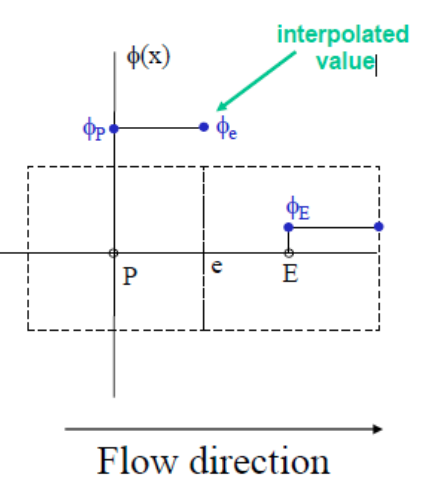
\includegraphics[scale = 0.56]{7.png}
  \caption{first order upwind scheme }
  \label{fig:1st upwind scheme }
\end{figure}
\noindent (一、1.1)定義符號:\\
\begin{equation}\
    \begin{split}
        (1)&\mbox{相臨計算點溫度定義(對於各個計算點):}\\
        &T_{i,j}\ = T_{p}\\
        &T_{i-1,j}\ = T_{W} \\
        &T_{i+1,j}\ = T_{E} \\
        (2)&\mbox{邊界計算點的特殊邊界中心點的溫度:}\\
        &T_{-\frac{1}{2},j}\ ,T_{Nx-\frac{1}{2},j}\\
        (3)&\mbox{西邊界中心點的擴散符號$D_{w}$:(對於計算點(i = 1 : Nx-1))}\\
        &\mbox{計算點(i = 1 : Nx-1)的西邊界中心點的擴散符號:}\\
        &A_{w}\cdot \frac{\alpha_{i,j}+\alpha_{i-1,j}}{2}\cdot \frac{1}{\Delta x_{pW}} = D_{w}\\
        &\mbox{東邊界中心點的擴散符號$D_{e}$:(對於計算點(i = 0 : Nx-2))}\\
        &\mbox{計算點(i = 0 : NX-2)的東邊界中心點的擴散符號:}\\
        &A_{e}\cdot \frac{\alpha_{i+1,j}+\alpha_{i,j}}{2}\cdot \frac{1}{\Delta x_{Ep}} = D_{e}\\
        &\mbox{擴散符號需要在特殊邊界討論}\\
        &\mbox{(3.1)西邊界中心點的擴散符號$D_{w}^{*}$:(對於左邊界計算點(i = 0))}\\
        &\mbox{左邊界計算點的西邊界中心點的擴散符號:(均勻網格)}\\
        &A_{w}\cdot \alpha_{-\frac{1}{2},j} \cdot \frac{1}{\Delta x_{pw}} = D_{l} = D_{w}^{*}\\
        &\mbox{(3.2)東邊界中心點的擴散符號$D_{e}^{*}$:(對於右邊界計算點(i = Nx-1))}\\
        &\mbox{右邊界計算點的東邊界中心點的擴散符號:(均勻網格)}\\
        &A_{e}\cdot \alpha_{Nx-\frac{1}{2},j} \cdot \frac{1}{\Delta x_{ep}} = D_{r} = D_{e}^{*}\\
        (4)&\mbox{各邊界中心點的對流符號的定義:(對於計算點(i = 0:Nx-1))}\\
        &\mbox{對流符號不需在特殊邊界討論}\\
        &\mbox{西邊界中心點的對流符號$F_{w}$:(對於計算點(i = 0 : Nx-1))}\\
        &\mbox{計算點(i = 0 : Nx-1)的西邊界中心點的對流符號:}\\
        &A_{w}\cdot u_{x\ i+\frac{1}{2},j} = F_{w}\\
        &\mbox{東邊界中心點的對流符號$F_{e}$:(對於計算點(i = 0 : Nx-1))}\\
        &\mbox{計算點(i = 0 : Nx-1)的東邊界中心點的對流符號:}\\
        &A_{e}\cdot u_{x\ i-\frac{1}{2},j} = F_{e}\\
        (5)&\mbox{離散方程中,對應西側計算點的組合係數$a_{W}$:(對於計算點(i = 1 : Nx-1))}\\    
        &\mbox{對應計算點(i = 2 : Nx)的西側計算點的組合係數:}\\
        &a_{W} = D_{w} + max(F_{w},0)\\
        &\mbox{離散方程中,對應東側計算點的組合係數$a_{E}$:(對於計算點(i = 0 : Nx-2))}\\
        &\mbox{對應計算點(i = 0 : Nx-2)的東側計算點的組合係數:}\\
        &a_{E} = D_{e} - min(0,F_{e}) \\
        &\mbox{離散方程中,對應本計算點的組合係數$a_{p}$:(對於計算點(i = 1 : Nx-2))}\\    
        &\mbox{對應計算點(i = 1 : Nx-2)的組合係數:}\\
        &a_{p} = a_{W}-F_{e} + a_{E} + F_{e} \\
    \end{split}
\end{equation}
\newpage
\noindent (一、1.2)迎風討論(主要討論內部計算點(i = 1 : Nx-2)):\\

\noindent (1)若且唯若$u_{x\ i-\frac{1}{2} , j} > 0$,則\\
    離散方程中,對應西側計算點的線組係數$a_{W}$:
    (對於計算點(i = 1 : Nx-1))\\
    對應計算點(i = 1 : Nx-1)的西側計算點的線組係數:\\
    $$a_{W} = D_{w} \rightarrow D_{w} + F_{w}$$\\
    離散方程中,對應本計算點的線組係數$a_{p}$:
    (對於計算點(i = 1 : Nx-1))\\
    對應計算點(i = 1 : Nx-1)的的線組係數:\\
    $$a_{p} : D_{w} \rightarrow D_{w}$$\\
\noindent 則:\\
\begin{equation}
    \begin{split}
    a_{p} = a_{W} - F_{W} ...
\end{split}
\end{equation}

\noindent (2)若且唯若$u_{x\ i-\frac{1}{2} , j} < 0$,則\\
    離散方程中,對應西側計算點的線組係數$a_{W}$:
    (對於計算點(i = 1 : Nx-1))\\
    對應計算點(i = 1 : Nx-1)的西側計算點的線組係數:\\
    $$a_{W} = D_{w} \rightarrow D_{w} $$\\
    離散方程中,對應本計算點的線組係數$a_{p}$:
    (對於計算點(i = 1 : Nx-1))\\
    對應計算點(i = 1 : Nx-1)的的線組係數:\\
    $$a_{p} : D_{w} \rightarrow D_{w} -F_{w}$$\\
\noindent 則:\\
\begin{equation}
    a_{p} = a_{W} - F_{W} ...
\end{equation}

\noindent (3)若且唯若$u_{x\ +\frac{1}{2} , j} > 0$,則\\
    離散方程中,對應東側計算點的線組係數$a_{E}$:
    (對於計算點(i = 0 : Nx-2))\\
    對應計算點(i = 0 : Nx-2)的東側計算點的線組係數:\\
    $$a_{E} = D_{e} \rightarrow D_{e} $$\\
    離散方程中,對應本計算點的線組係數$a_{p}$:
    (對於計算點(i = 0 : Nx-2))\\
    對應計算點(i = 0 : Nx-2)的的線組係數:\\
    $$a_{p} : D_{w} \rightarrow D_{w} + F_{e}$$\\
\noindent 則:\\
\begin{equation}
    a_{p} = a_{E} + F_{e} ...
\end{equation}

\noindent (4)若且唯若$u_{x\ i+\frac{1}{2} , j} < 0$,則\\
    離散方程中,對應西側計算點的線組係數$a_{W}$:
    (對於計算點(i = 0 : Nx-2))\\
    對應計算點(i = 0 : Nx-2)的西側計算點的線組係數:\\
    $$a_{E} = D_{e} \rightarrow D_{e} - F_{e}$$\\
    離散方程中,對應本計算點的線組係數$a_{p}$:
    (對於計算點(i = 0 : Nx-2))\\
    對應計算點(i = 0 : Nx-2)的的線組係數:\\
    $$a_{p} : D_{e} \rightarrow D_{e}$$\\
\noindent 則:\\
\begin{equation}
    a_{p} = a_{E} + F_{e} ...
\end{equation}

\noindent (5)最終結論:\\

\noindent 離散方程中,對應西側計算點的線組係數$a_{W}$:
    (對於計算點(i = 1 : Nx-1))\\
    對應計算點(i = 1 : Nx-1)的西側計算點的線組係數:\\
\begin{equation}a_{W}  = D_{w} + max(F_{w},0)\end{equation}\\
    離散方程中,對應東側計算點的線組係數$a_{E}$:
    (對於計算點(i = 0 : Nx-2))\\
    對應計算點(i = 0 : Nx-2)的東側計算點的線組係數:\\
\begin{equation}a_{E}  = D_{e} - min(0,F_{e})\end{equation}\\
    離散方程中,對應本計算點的線組係數$a_{p}$:
    (對於計算點(i = 1 : Nx-2))\\
    對應計算點(i = 1 : Nx-2)的的線組係數:\\
\begin{equation}a_{p}  = (a_{W} - F_{w}) + (a_{E} + F_{e}) \end{equation}\\

\noindent (一、1.3)內計算點離散方程:\\
不可壓縮理想氣體的一維穩態擴散對流方程的空間一階精度upwind離散格式:(對於計算點(i = 1 : Nx-2))\\
計算點(i = 1 : Nx-2)的不可壓縮理想氣體的一維穩態擴散對流方程的空間一階精度upwind離散格式:\\
\begin{equation}
\begin{split}
    a_{p}T_{p} = a_{W}T_{W} + a_{E}T_{E}\\
\end{split}
\end{equation}
\noindent 其中,
\begin{equation}
    \begin{split}
        &a_{p} = (a_{W} - F_{w}) + (a_{E} + F_{e})\\
        &a_{W} = D_{w} + max(F_{w},0)\\
        &a_{E} = D_{e} - min(0 , F_{e})\\
    \end{split}
\end{equation}
\noindent (一、1.4)邊界計算點定義符號 :\\
\begin{equation}
    \begin{split}
        (1)left\ &node \\
        &\mbox{離散方程中,對應西側計算點的線組係數$a_{W}^{*}$:(對於左邊界計算點(i = 0))}\\    
        &\mbox{對應左邊界計算點的西側計算點的線組係數:}\\
        &a_{W}^{*} = 0\\
        &\mbox{離散方程中,等左外源項$S_{pl}^{*}$:對於左計算點(i = 0)}\\
        &\mbox{左邊界計算點的等左外源項:}\\
        &S_{pl}^{*} = D_{w}^{*} + max(F_{w},0) \\
        &\mbox{離散方程中,對應本計算點的線組係數$a_{pl}^{*}$:(對於左邊界計算點(i = 0))}\\    
        &\mbox{對應左邊界計算點的線組係數:}\\
        &a_{pl}^{*} = (a_{W}^{*}-F_{w}) + (a_{E} + F_{e}) + S_{pl}^{*} \\
        &\mbox{離散方程中,等右外源項$S_{ul}^{*}$:(對於左邊界計算點(i = 0))}\\
        &\mbox{左邊界計算點的等右外源項:}\\
        &S_{ul}^{*} = (D_{w}^{*}  + max( F_{w} , 0 ))\cdot T_{l}\\
\end{split}
\end{equation}
\begin{equation}
    \begin{split}
        (2)right\ &node \\
        &\mbox{離散方程中,對應東側計算點的線組係數$a_{E}^{*}$:(對於右邊界計算點(i = Nx-1))}\\    
        &\mbox{對應右邊界計算點的東側計算點的線組係數:}\\
        &a_{E}^{*} = 0\\
        &\mbox{離散方程中,等左外源項$S_{pl}^{*}$:對於右計算點(i = Nx-1)}\\
        &\mbox{右邊界計算點的等左外源項:}\\
        &S_{pr}^{*} = D_{e}^{*} -min(0,F_{e}) \\
        &\mbox{離散方程中,對應本計算點的線組係數$a_{pr}^{*}$:(對於右邊界計算點(i = Nx-1))}\\    
        &\mbox{對應右邊界計算點的線組係數:}\\
        &a_{pr}^{*} = (a_{W}-F_{w}) + (a_{E}^{*} + F_{e}) + S_{pr}^{*} \\
        &\mbox{離散方程中,等右外源項$S_{ul}^{*}$:(對於右邊界計算點(i = Nx-1))}\\
        &\mbox{右邊界計算點的等右外源項:}\\
        &S_{ur}^{*} = (D_{e}^{*}  - min(0 , F_{e} ))\cdot T_{r}\\
\end{split}
\end{equation}

\vspace{0.7em}

\noindent (一、1.5)左邊界計算點迎風討論 :\\

\noindent (1-1)若且唯若$u_{x\ -\frac{1}{2} ,j} > 0$ ,則:\\
離散方程中,對應西側計算點的線組係數$a_{W}^{*}$:(對於左計算點(i = 0))\\
對應左邊界計算點的西側計算點的線組係數:\\
$$a_{W}^{*} = 0$$\\
離散方程中,對應本計算點的線組係數$a_{pl}^{*}$:(對於左邊界計算點(i = 0))\\
對應左邊界計算點的線組係數:\\
$$a_{pl}^{*} : D_{w}^{*} - F_{w} \rightarrow D_{w}^{*}$$\\
離散方程中,等右外源項$S_{ul}^{*}$:(對於左邊界計算點(i = 0))\\
左邊界計算點的等右外源項:\\
$$S_{ul}^{*} = D_{w}^{*} \rightarrow D_{w}^{*}+F_{w}$$\\

\noindent (1-2)
        在\\
        離散方程中,對應本計算點的線組係數$a_{pl}^{*}$:(對於左邊界計算點(i = 0))\\    
        對應左邊界計算點的線組係數:\\
        $$a_{pl}^{*} = (a_{W}^{*}-F_{w}) + (a_{E} + F_{e}) + S_{pl}^{*}$$\\
        下,\\
        若且唯若\\
        離散方程中,對應本計算點的線組係數$a_{pl}^{*}$:(對於左邊界計算點(i = 0))\\
        對應左邊界計算點的線組係數:\\
        $$a_{pl}^{*} : D_{w}^{*} - F_{w} \rightarrow D_{w}^{*}$$\\
        則:\\
        離散方程中,等左外源項$S_{pl}^{*}$:(對於左邊界計算點(i = 0))\\
        左邊界計算點的等左外源項:\\
        \begin{equation}
        S_{pl}^{*} = D_{w}^{*} \rightarrow D_{w}^{*}+F_{w}
        \end{equation}


\noindent (2-1)若且唯若$u_{x\ -\frac{1}{2} ,j} < 0$ ,則:\\
離散方程中,對應西側計算點的線組係數$a_{W}^{*}$:(對於左計算點(i = 0))\\
對應左邊界計算點的西側計算點的線組係數:\\
$$a_{W}^{*} = 0$$\\
離散方程中,對應本計算點的線組係數$a_{pl}^{*}$:(對於左邊界計算點(i = 0))\\
對應左邊界計算點的線組係數:\\
$$a_{pl}^{*} : D_{w}^{*} - F_{w} \rightarrow D_{w}^{*} - F_{w}$$\\
離散方程中,等右外源項$S_{ul}^{*}$:(對於左邊界計算點(i = 0))\\
左邊界計算點的等右外源項:\\
$$S_{ul}^{*} = D_{w}^{*} \rightarrow D_{w}^{*}$$\\

\noindent (2-2)
        在\\
        離散方程中,對應本計算點的線組係數$a_{pl}^{*}$:(對於左邊界計算點(i = 0))\\    
        對應左邊界計算點的線組係數:\\
        $$a_{pl}^{*} = (a_{W}^{*}-F_{w}) + (a_{E} + F_{e}) + S_{pl}^{*}$$\\
        下,\\
        若且唯若\\
        離散方程中,對應本計算點的線組係數$a_{pl}^{*}$:(對於左邊界計算點(i = 0))\\
        對應左邊界計算點的線組係數:\\
        $$a_{pl}^{*} : D_{w}^{*} - F_{w} \rightarrow D_{w}^{*} - F_{w}$$\\
        則:\\
        離散方程中,等左外源項$S_{pl}^{*}$:(對於左邊界計算點(i = 0))\\
        左邊界計算點的等左外源項:\\
        \begin{equation}
        S_{pl}^{*} = D_{w}^{*} \rightarrow D_{w}^{*}\\
        \end{equation}
\noindent (3)若且唯若$u_{x\ +\frac{1}{2} ,j} > 0$ ,則:\\
離散方程中,對應東側計算點的線組係數$a_{E}$:(對於左計算點(i = 0))\\
對應左邊界計算點的東側計算點的線組係數:\\
$$a_{E} = D_{e} \rightarrow D_{e}$$\\
離散方程中,對應本計算點的線組係數$a_{pl}^{*}$:(對於左邊界計算點(i = 0))\\
對應左邊界計算點的線組係數:\\
$$a_{pl}^{*} : D_{e} \rightarrow D_{e} + F_{e}$$\\
\noindent 則:\\
\begin{equation}a_{pl}^{*} : a_{E} + F_{e} +\cdots\end{equation}\\


\noindent (4)若且唯若$u_{x\ +\frac{1}{2} ,j} < 0$ ,則:\\
離散方程中,對應東側計算點的線組係數$a_{E}$:(對於左計算點(i = 0))\\
對應左邊界計算點的東側計算點的線組係數:\\
$$a_{E} = D_{e} \rightarrow D_{e} - F_{e}$$\\
離散方程中,對應本計算點的線組係數$a_{pl}^{*}$:(對於左邊界計算點(i = 0))\\
對應左邊界計算點的線組係數:\\
$$a_{pl}^{*} : D_{e} \rightarrow D_{e} $$\\
\noindent 則:\\
\begin{equation}a_{pl}^{*} : a_{E} + F_{e} +\cdots\end{equation}\\

\noindent (5)最終結論:\\
離散方程中,等右外源項$S_{pl}^{*}$:(對於左邊界計算點(i = 0))\\
左邊界計算點的等右外源項:\\
\begin{equation}
    \begin{split}
        S_{ul}^{*} = D_{w}^{*} + max(F_{w},0)\\
    \end{split}
\end{equation}
\noindent 離散方程中,對應東側計算點的線組係數$a_{E}$:(對於左計算點(i = 0))\\
對應左邊界計算點的東側計算點的線組係數:\\
\begin{equation}
    \begin{split}
        a_{E} = D_{e} - min(0,F_{e})\\
    \end{split}
\end{equation}
\noindent 離散方程中,對應本計算點的線組係數$a_{pl}^{*}$:(對於左邊界計算點(i = 0))\\
對應左邊界計算點的線組係數:\\
\begin{equation}
    \begin{split}
        a_{pl}^{*} = (a_{W}^{*}-F_{w}) + (a_{E} + F_{e}) + S_{pl}^{*}\\
    \end{split}
\end{equation}
\noindent 離散方程中,等左外源項$S_{pl}^{*}$:(對於左邊界計算點(i = 0))\\
左邊界計算點的等左外源項:\\
\begin{equation}
    S_{pl}^{*} = D_{w}^{*} + max(F_{w},0)\\
\end{equation}
\noindent (一、1.6)右邊界計算點迎風討論 :\\


\noindent (1-1)若且唯若$u_{x\ Nx-\frac{1}{2} ,j} > 0$ ,則:\\
離散方程中,對應東側計算點的線組係數$a_{E}^{*}$:(對於右邊界計算點(i = Nx-1))\\
對應右邊界計算點的西側計算點的線組係數:\\
$$a_{E}^{*} = 0$$\\
離散方程中,對應本計算點的線組係數$a_{pr}^{*}$:(對於右邊界計算點(i = Nx-1))\\
對應右邊界計算點的線組係數:\\
$$a_{pr}^{*} : D_{E}^{*} + F_{e} \rightarrow D_{E}^{*} + F_{e}$$\\
離散方程中,等右外源項$S_{ur}^{*}$:(對於右邊界計算點(i = Nx-1))\\
右邊界計算點的等右外源項:\\
$$S_{ur}^{*} = D_{E}^{*} \rightarrow D_{E}^{*} $$\\

\noindent (1-2)
        在\\
        離散方程中,對應本計算點的線組係數$a_{pr}^{*}$:(對於右邊界計算點(i = Nx-1))\\
        對應右邊界計算點的線組係數:\\
        $$a_{pr}^{*} = (a_{W}-F_{w}) + (a_{E}^{*} + F_{e}) + S_{pr}^{*}$$\\
        下,\\
        若且唯若\\
        離散方程中,對應本計算點的線組係數$a_{pr}^{*}$:(對於右邊界計算點(i = Nx-1))\\
        對應右邊界計算點的線組係數:\\
        $$a_{pr}^{*} : D_{E}^{*} + F_{e} \rightarrow D_{E}^{*} + F_{e}$$\\
        則:\\
        離散方程中,等左外源項$S_{pr}^{*}$:(對於右邊界計算點(i = Nx-1))\\
        右邊界計算點的等左外源項:\\
        \begin{equation}
        S_{pr}^{*} = D_{E}^{*} \rightarrow D_{E}^{*}\\
        \end{equation}


\noindent (2-1)若且唯若$u_{x\ Nx-\frac{1}{2} ,j} < 0$ ,則:\\
離散方程中,對應東側計算點的線組係數$a_{E}^{*}$:(對於右邊界計算點(i = Nx-1))\\
對應右邊界計算點的西側計算點的線組係數:\\
$$a_{E}^{*} = 0$$\\
離散方程中,對應本計算點的線組係數$a_{pr}^{*}$:(對於右邊界計算點(i = Nx-1))\\
對應右邊界計算點的線組係數:\\
$$a_{pr}^{*} : D_{E}^{*} + F_{e} \rightarrow D_{E}^{*} $$\\
離散方程中,等右外源項$S_{ur}^{*}$:(對於右邊界計算點(i = Nx-1))\\
右邊界計算點的等右外源項:\\
$$S_{ur}^{*} = D_{E}^{*} \rightarrow D_{E}^{*} - F_{e} $$\\

\noindent (2-2)
        在\\
        離散方程中,對應本計算點的線組係數$a_{pr}^{*}$:(對於右邊界計算點(i = Nx-1))\\    
        對應右邊界計算點的線組係數:\\
        $$a_{pr}^{*} = (a_{W}-F_{w}) + (a_{E}^{*} + F_{e}) + S_{pr}^{*}$$\\
        下,\\
        若且唯若\\
        離散方程中,對應本計算點的線組係數$a_{pr}^{*}$:(對於右邊界計算點(i = Nx-1))\\
        對應右邊界計算點的線組係數:\\
        $$a_{pr}^{*} :D_{E}^{*} + F_{e} \rightarrow D_{E}^{*} $$\\
        則:\\
        離散方程中,等左外源項$S_{pr}^{*}$:(對於右邊界計算點(i = Nx-1))\\
        右邊界計算點的等左外源項:\\
        \begin{equation}
        S_{pr}^{*} = D_{E}^{*} \rightarrow D_{E}^{*} - F_{e}\\
        \end{equation}

\noindent (3)若且唯若$u_{x\ Nx-\frac{3}{2} ,j} > 0$ ,則:\\
離散方程中,對應西側計算點的線組係數$a_{W}$:(對於右邊界計算點(i = Nx-1))\\
對應右邊界計算點的西側計算點的線組係數:\\
$$a_{W} = D_{w} \rightarrow D_{w} + F_{w}$$\\
離散方程中,對應本計算點的線組係數$a_{pr}^{*}$:(對於右邊界計算點(i = Nx-1))\\
對應右邊界計算點的線組係數:\\
$$a_{pr}^{*} : D_{w} \rightarrow D_{w}$$\\
\noindent 則:\\
\begin{equation}a_{pr}^{*} : a_{W} - F_{w} +\cdots\end{equation}\\


\noindent (4)若且唯若$u_{x\ Nx-\frac{3}{2} ,j} < 0$ ,則:\\
離散方程中,對應西側計算點的線組係數$a_{W}$:(對於右邊界計算點(i = Nx-1))\\
對應右邊界計算點的西側計算點的線組係數:\\
$$a_{W} = D_{w} \rightarrow D_{w} $$\\
離散方程中,對應本計算點的線組係數$a_{pr}^{*}$:(對於右邊界計算點(i = Nx-1))\\
對應右邊界計算點的線組係數:\\
$$a_{pr}^{*} : D_{w} \rightarrow D_{w} - F_{w}$$\\
\noindent 則:\\
\begin{equation}a_{pr}^{*} : a_{W} - F_{w} +\cdots\end{equation}\\

\noindent (5)最終結論:\\
離散方程中,等右外源項$S_{pr}^{*}$:(對於右邊界計算點(i = Nx-1))\\
右邊界計算點的等右外源項:\\
\begin{equation}
    \begin{split}
        S_{ur}^{*} = D_{e}^{*} -min(0,F_{e})\\
    \end{split}
\end{equation}
\noindent 離散方程中,對應西側計算點的線組係數$a_{W}$:(對於右邊界計算點(i = Nx-1))\\
對應左邊界計算點的西側計算點的線組係數:\\
\begin{equation}
    \begin{split}
        a_{W} = D_{w} + max(F_{w} , 0)\\
    \end{split}
\end{equation}
\noindent 離散方程中,對應本計算點的線組係數$a_{pr}^{*}$:(對於右邊界計算點(i = Nx-1))\\
對應右邊界計算點的線組係數:\\
\begin{equation}
    \begin{split}
        a_{pr}^{*} = (a_{W}-F_{w}) + (a_{E}^{*} + F_{e}) + S_{pr}^{*}\\
    \end{split}
\end{equation}
\noindent 離散方程中,等左外源項$S_{pr}^{*}$:(對於右邊界計算點(i = Nx-1))\\
右邊界計算點的等左外源項:\\
\begin{equation}
    S_{pr}^{*} =  D_{e}^{*} -min(0,F_{e})\\
\end{equation}
\newpage 

\noindent (一、1.7)左邊界計算點離散方程:\\

\noindent 不可壓縮理想氣體的一維穩態擴散對流方程的空間一階精度upwind離散格式:(對於左邊界計算點(i = 0))\\
左邊界計算點的不可壓縮理想氣體的一維穩態擴散對流方程的空間一階精度upwind離散格式:\\
\begin{equation}
    \begin{split}
        a_{pl}^{*}T_{p} = a_{W}^{*}T_{W} + a_{E}T_{E} + S_{ul}^{*}\\
    \end{split}
\end{equation}
\noindent 其中,
\begin{equation}
    \begin{split}
        &a_{pl}^{*} = (a_{W}^{*}-F_{w}) + (a_{E} + F_{e}) + S_{pl}^{*} \\
        &a_{W}^{*} = 0 \\
        &a_{E} = D_{e} - min(0,F_{e})\\
        &S_{pl}^{*} = D_{w}^{*} + max(F_{w},0) \\
        &S_{ul}^{*} = (D_{w}^{*} + max(F_{w},0))\cdot T_{l} \\
    \end{split}
\end{equation}
\noindent (一、1.8)右邊界計算點離散方程:\\

\noindent 不可壓縮理想氣體的一維穩態擴散對流方程的空間一階精度upwind離散格式:(對於右邊界計算點(i = Nx-1))\\
右邊界計算點的不可壓縮理想氣體的一維穩態擴散對流方程的空間一階精度upwind離散格式:\\
\begin{equation}
    \begin{split}
        a_{pr}^{*}T_{p} = a_{W}T_{W} + a_{E}^{*}T_{E} + S_{ur}^{*}\\
    \end{split}
\end{equation}
\noindent 其中,
\begin{equation}
    \begin{split}
        &a_{pr}^{*} = (a_{W}-F_{w}) + (a_{E}^{*} + F_{e}) + S_{pr}^{*} \\
        &a_{W} = D_{w} + max(F_{w},0) \\
        &a_{E}^{*} = 0 \\
        &S_{pr}^{*} = D_{e}^{*} - min(0,F_{e}) \\
        &S_{pr}^{*} = (D_{e}^{*}  - min(0 , F_{e} ))\cdot T_{r}\\
    \end{split}
\end{equation}
\end{document}


